\documentclass[12pt,a4paper]{article}
\usepackage[utf8]{inputenc}
\usepackage[T1]{fontenc}
\usepackage[version=4]{mhchem}
\usepackage{stix2}

\usepackage[german]{authblk}
\author[1]{Mika Riesterer}

\affil[1]{Labor 9, Gruppe 5, Platz 45, Assistent: Xiqin Pu}

\usepackage[margin=2cm,includeheadfoot]{geometry}

\usepackage{parskip}

\renewcommand{\topfraction}{1}

\usepackage[german]{babel}

\usepackage{fancyhdr}
\pagestyle{fancy}
\fancyhf{}

\setlength{\headheight}{15pt}

\fancyhead[L]{Stand: \today}
\fancyhead[C]{2,4-Dimethylacetophenon}
\fancyhead[R]{Seite \thepage}

\usepackage{amsmath}
\usepackage{wasysym}
\usepackage{graphicx}
\usepackage{textcomp, gensymb}

\usepackage{subfig}

\usepackage{csquotes}
\usepackage[backend=bibtex]{biblatex}
\addbibresource{refs.bib}
\setcounter{biburlnumpenalty}{9000} % Umbruch nach Zahlen
\setcounter{biburlucpenalty}{9000}  % Umbruch nach Großbuchstaben
\setcounter{biburllcpenalty}{9000}  % Umbruch nach Kleinbuchstaben

\usepackage{siunitx}
\sisetup{
  per-mode=fraction,
  fraction-function=\tfrac
}

\usepackage[hidelinks]{hyperref}
\usepackage{color}
\usepackage{colortbl}
\usepackage{float}
\definecolor{gray}{gray}{0.75}
\definecolor{gray5}{gray}{0.5}

\setlength{\emergencystretch}{10pt}

\usepackage{caption}
\captionsetup{format=hang,labelfont=it,textfont=it}

\newcommand*{\vv}[1]{\overrightarrow{\mkern0mu#1}}

\newcommand{\specialcell}[2][c]{%
\begin{tabular}[#1]{@{}c@{}}#2\end{tabular}}

\begin{document}
\pagenumbering{Roman}

% Change here
\title{%
    Präparat 1 (2,4-Dimethylacetophenon) \\
    \large Friedel-Crafts-Acylierung \\[0.5cm]
    \begin{figure}[H]
      \centering
      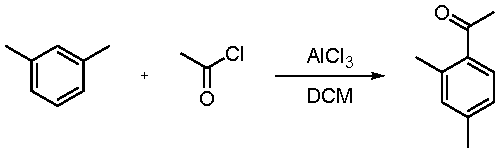
\includegraphics[width=0.7\textwidth]{drawings/P1.pdf} \\[0.5cm]
      \caption{Reaktiongleichung der Friedel-Crafts-Acylierung}
      \label{fig:P1}
    \end{figure}
    \large Organisch-chemisches Grundpraktikum - SoSe 2026 \\
    \large Versuchsdurchführung am 27.04. - 05.05.2026}

\date{\today}

\maketitle
\thispagestyle{empty}
\newpage

\pagenumbering{arabic}

\section{Einleitung}
Die Herstellung des Präparats Benzyltriphenylphosphoniumbromid erfolgt über eine Alkylierung von tertiären Phosphinen nach der Vorschrift des Organikums \cite{ROV}. \newline
Das Edukt Triphenylphosphan reagiert mit Benzylbromid unter dem Lösungsmittel Toluol (Abb. \ref{fig:P3}). \newline
Benzyltriphenylphosphoniumbromid beziehungsweise andere Phosphorylide können als Edukte für die bekannte Wittig-Reaktion verwendet werden. Es bilden sich dadurch (E)-/(Z)-Alkene \cite{ORG}.

\section{Mechanismus}
Bei der Friedel-Crafts-Acylierung handelt es sich um eine elektrophile aromatische Substitution ($S_E\text{Ar}$) \cite{ROV}. 

Zunächst wird das Acetylchlorid durch die Lewis-Säure $\ce{AlCl3}$ aktiviert. 
Unter Abspaltung eines Chlorid-Ions entstehen ein stark elektrophiles Acylium-Ion und ein $\ce{AlCl4-}$-Komplex. 
Der nukleophile Angriff des $\pi$-Systems des Aromaten am Acylium-Ion hebt den aromatischen Zustand temporär auf und führt zur Bildung eines mesomeriestabilisierten Wheland-Komplexes. 

Die Rearomatisierung erfolgt durch Deprotonierung: 
Ein Chlorid-Ion des $\ce{AlCl4-}$ abstrahiert das Proton am $sp^3$-hybridisierten Ringkohlenstoff, wodurch unter Freisetzung von $\ce{HCl}$ das aromatische System wiederhergestellt wird. 
Da die basische Carbonylgruppe des entstandenen 2,4-Dimethylacetophenons einen stabilen Komplex mit dem $\ce{AlCl3}$ bildet, muss das Produkt im finalen Schritt durch wässrige Aufarbeitung zwingend hydrolytisch freigesetzt werden (Abb. \ref{fig:P1_M}).

\begin{figure}[H]
    \centering
    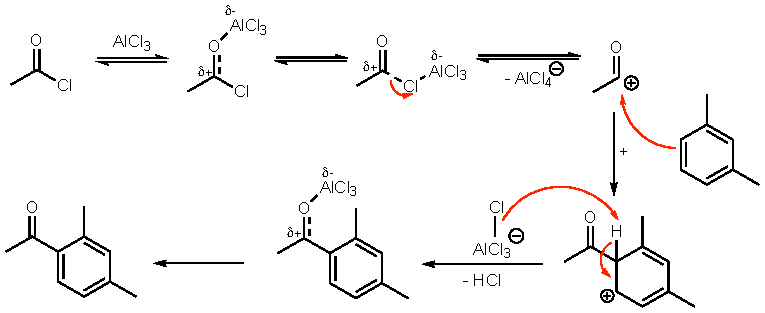
\includegraphics[width=1.0\textwidth]{drawings/P1_M.pdf} \\[0.5cm]
    \caption{Mechanismus der Friedel-Crafts-Acylierung von m-Xylol mit Acetylchlorid unter Aktivierung der Lewis-Säure Aluminiumchlorid im Lösungsmittel Dichlormethan.}
    \label{fig:P1_M}
\end{figure}

\section{Ergebnis}
Der Versuch wurde mit einer Ansatzgröße von \SI{50}{\milli\mole} Triphenylphosphan durchgeführt. 
Die Ausbeute an erhaltenem Rohprodukt nach Aufreinigung entspricht \SI{21.10}{\gram} (97\%).
Es liegt ein weißer Feststoff vor, welcher einen Schmelzpunkt \SI{296}{\degreeCelsius}--\SI{297}{\degreeCelsius} aufweist. Der Literaturwert wird mit \SI{295}{\degreeCelsius}--\SI{298}{\degreeCelsius} angegeben \cite{SA}. Die Reinheit beträgt >81.0\,\%.

\section{Diskussion}
Ursprünglich war ein Ansatz von \SI{50}{\milli\mole}, jedoch wurden zuvor die Werte für die Betriebsanweisung mit \SI{20}{\milli\mole} berechnet und im Nachhinein nicht mehr umgeändert. \newline
Die Abweichung des Brechungsindex vom Literaturwert ist mit $\approx 0.5\%$ sehr gering. 
Das Produkt 2,4-Dimethylacetophenon ist sehr gut isoliert, da im NMR (Abb. \ref{fig:P1_NMR}) bis auf eine Wasserverunreinigung bei $\delta = 1.70 ppm$, keinen nennenswerten Verunreinigungen zu sehen sind.
Ebenso bestätigt hat IR-Spektrum (Abb. \ref{fig:P1_IR}), dass das Produkt sehr rein vorliegt.

\section{Experiment}
\subsection{Allgemeines}
Die eingesetzten Reagenzien wurden von der zentralen Materialverwaltung bezogen. 
Das Kernresonanzspektrum wurde mit einem AV-250 der Fa. Bruker bei 300 K aufgenommen. \newline 
Die chemischen Verschiebungen sind in $\delta$-Werten (ppm) angegeben und beziehen sich für $^1H$-NMR-Spektren auf das Restprotonensignal des verwendeten Lösungsmittels \ce{CDCl3}. 
Bei der Zuordnung der Signale und für die Signalmultiplizitäten wurden die folgenden Abkürzungen verwendet: s – Singulett, bs – breites Singulett, d – Dublett, t – Triplett, q – Quartett, m – Multiplett.
Das IR-Spektrum wird mit einem Agilent Cary 630 FTIR gemessen. 

\subsection{Durchführung}
In einem Dreihalskolben wurden Styrol (\SI{5.21}{\gram}, \SI{50.0}{\milli\mole}), Chloroform (\SI{16.0}{\milli\liter}, \SI{200}{\milli\mole}), Benzyltriethylammoniumchlorid (\SI{0.114}{\gram}, \SI{0.50}{\milli\mole}) und Ethanol (\SI{0.5}{\milli\liter}) vorgelegt. 
Unter kräftigem Rühren wurde eiskalte, frisch bereitete 50\%ige Natronlauge (\SI{8.0}{\gram} NaOH in \SI{8.0}{\milli\liter} \ce{H2O}) zugegeben. 
Das zweiphasige Reaktionsgemisch wurde \SI{1}{\hour} bei Raumtemperatur und anschließend \SI{5}{\hour} bei \SI{50}{\degreeCelsius} gerührt.

Nach dem Abkühlen wurde das Gemisch in Wasser (\SI{250}{\milli\liter}) gegossen, die organische Phase abgetrennt und die wässrige Phase mit Chloroform (\SI{50}{\milli\liter}) extrahiert. 
Die vereinigten organischen Phasen wurden über wasserfreiem \ce{Na2SO4} getrocknet und filtriert. Es wurde mit weiteren \SI{50}{\milli\liter} Chloroform nachgespült. Das Lösungsmittel wurde am Rotationsverdampfer entfernt.
Das Rohprodukt wurde anschließend durch eine Vakuumdestillation gereinigt. 
Es wurde 1,1-Dichlor-2-phenylcyclopropan erhalten.

\section{Analytik}
\paragraph{Brechungsindex} $n_D(\SI{20}
{\degreeCelsius}) = 1.5343$ (Lit.: 1.535) \cite{SA1}.

\paragraph{NMR}
$^1$H-NMR (\SI{250}{\mega\hertz}, CDCl$_3$): $\delta$ = 7.64 (d, $^3J$ = \SI{8.5}{\hertz}, 1H, H-2), 7.10 -- 7.03 (m, 2H, H-3, H-5), 2.56 (s, 3H, H-10), 2.52 (s, 3H, H-8), 2.35 (s, 3H, H-7).

\begin{figure}[H]
    \centering
    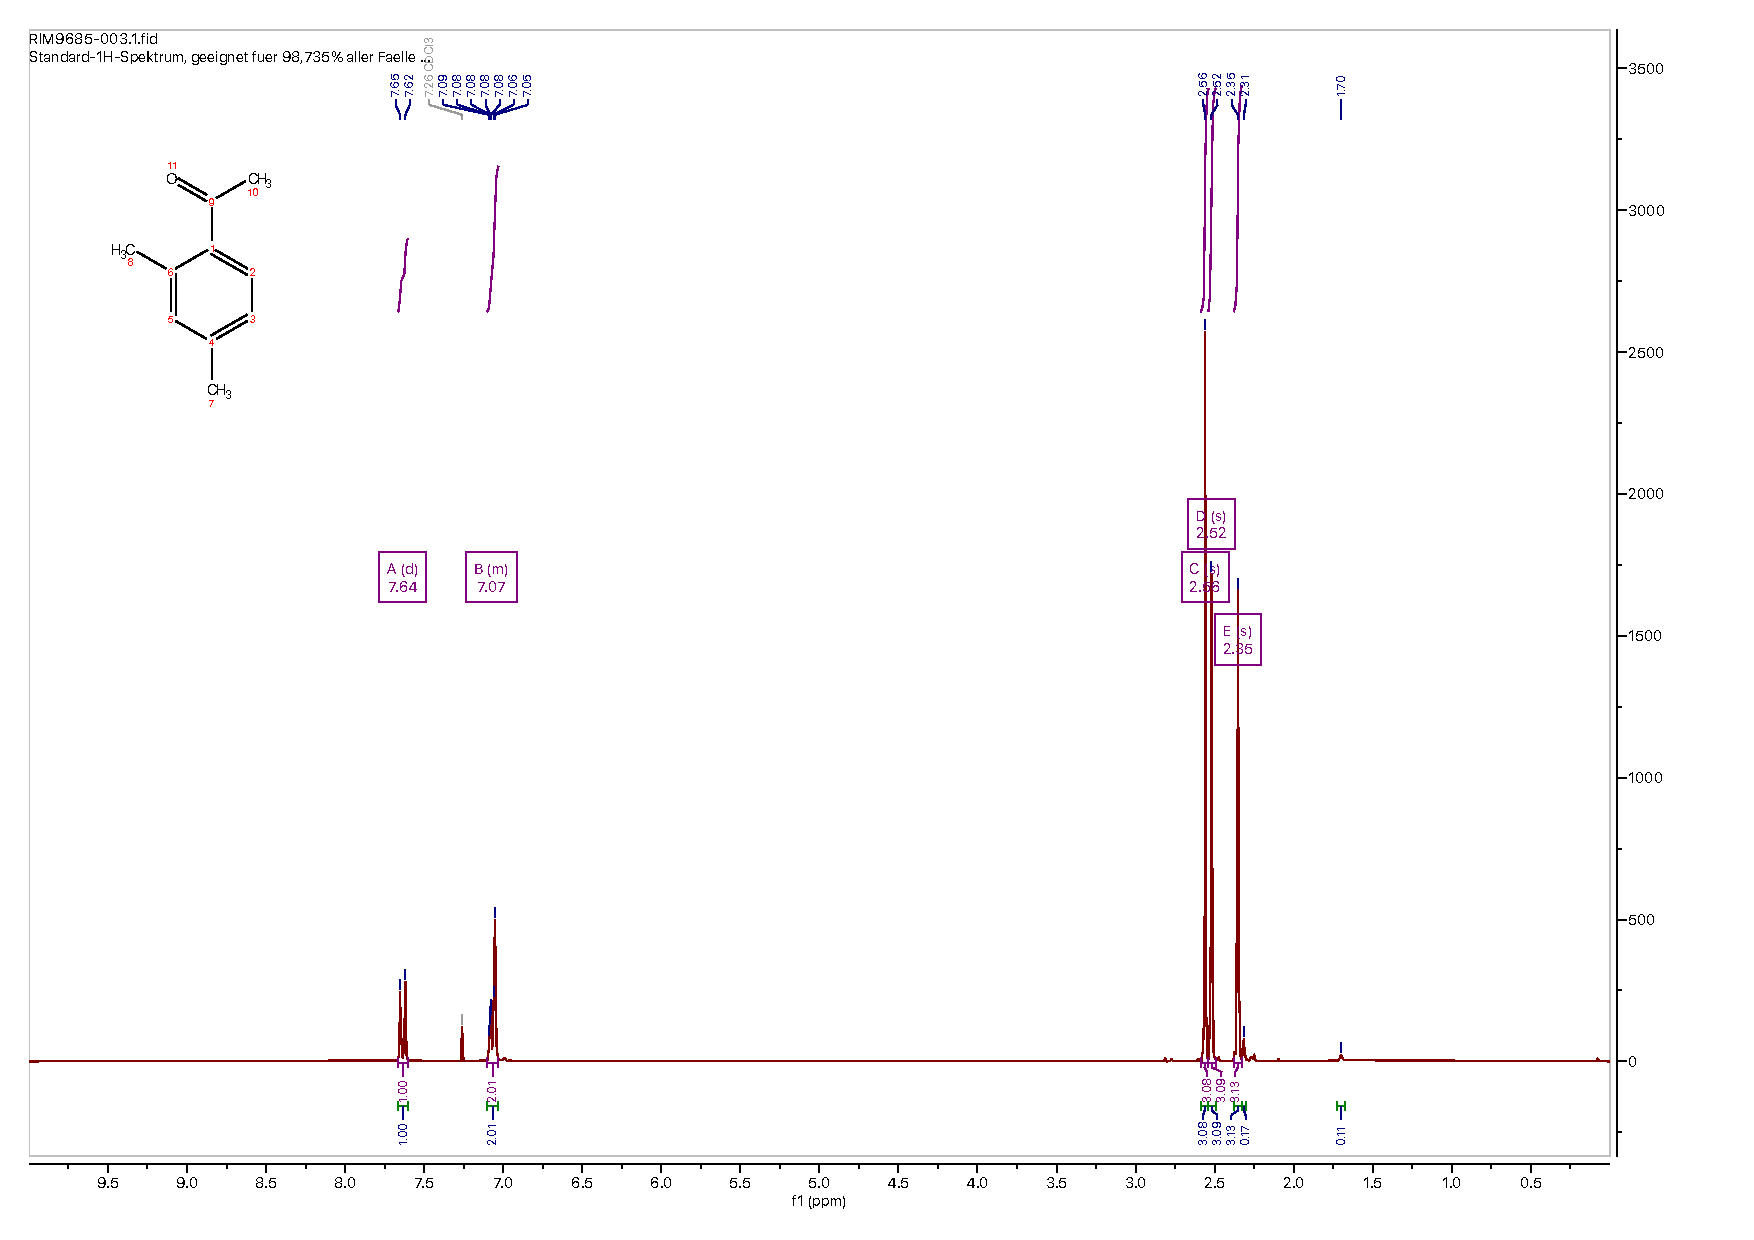
\includegraphics[width=1.0\textwidth]{data/P1_NMR.pdf} \\ [0.5cm]
    \caption{$^1H$-NMR Spektrum des erhaltenen Produkts 2,4-Dimethylacetophenon}
    \label{fig:P1_NMR}
\end{figure}

\paragraph{IR}
Das IR-Spektrum (Abbildung \ref{fig:P1_IR}) bestätigt die Struktur des erwünschten Produkts und passt zur Literatur \cite{SA2}.
Charakteristisch ist die intensive Carbonyl-Valenzschwingung bei $1675\,\text{cm}^{-1}$. Weitere signifikante Signale finden sich bei $2973$ und $2924\,\text{cm}^{-1}$ (aliphatische $C-H$-Valenz-schwingungen) sowie bei $1610$ und $1565\,\text{cm}^{-1}$ (aromatische $C=C$-Gerüstschwingungen). Die starke Bande bei $813\,\text{cm}^{-1}$ ($C-H$ out-of-plane) ist zudem typisch für einen 1,2,4-trisubstituierten Aromaten.


\begin{figure}[H]
    \centering
    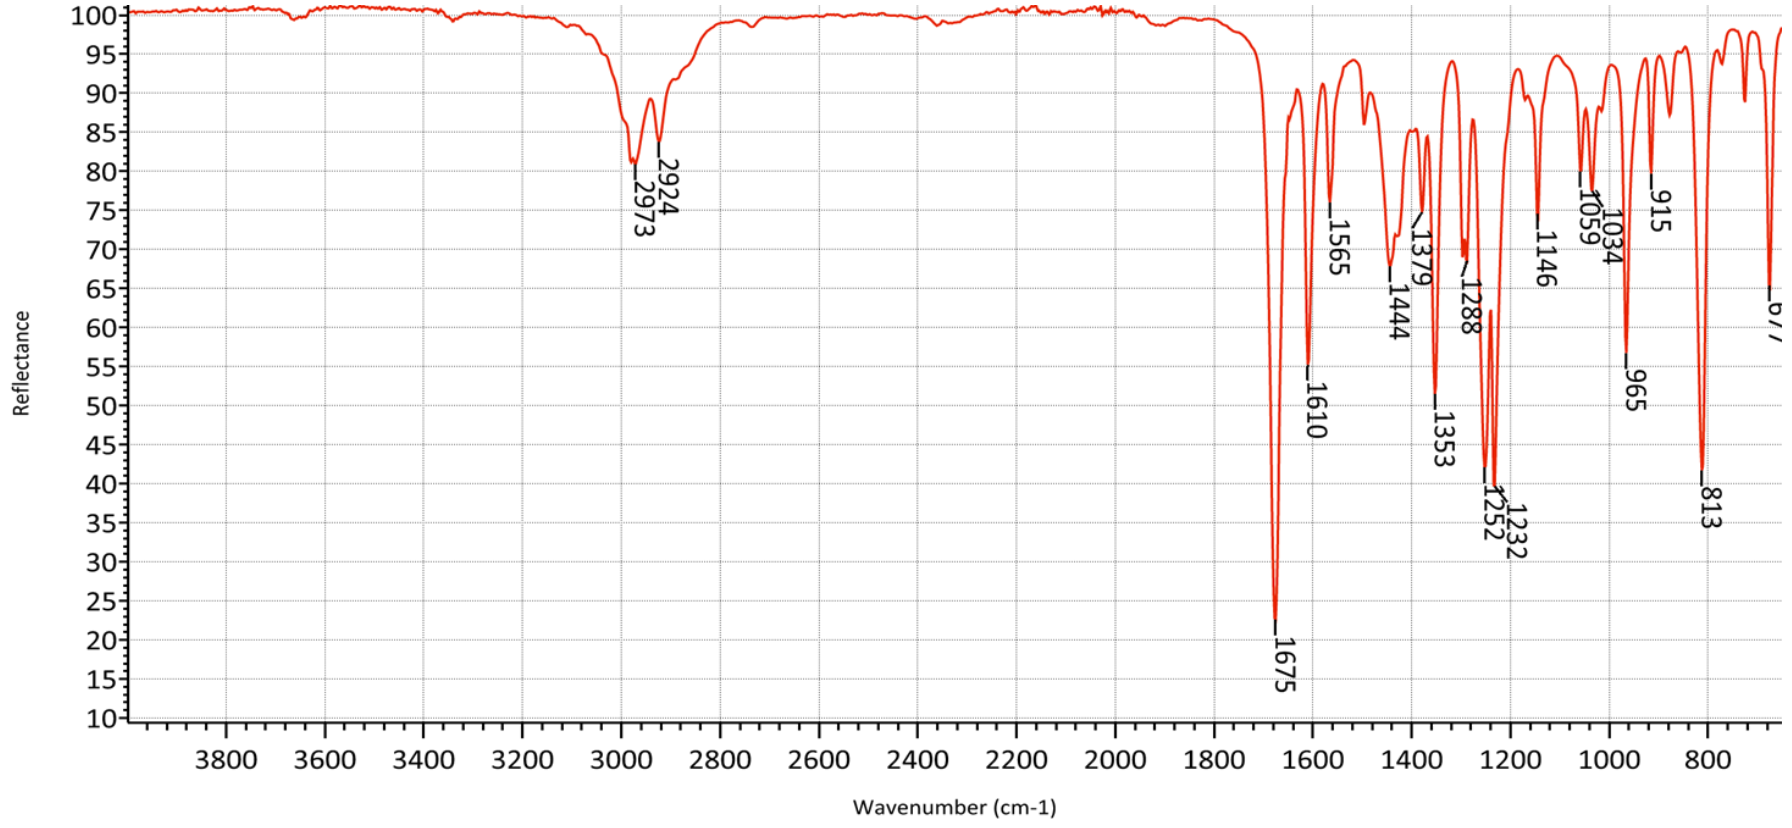
\includegraphics[width=1.0\textwidth]{data/P1_IR.png} \\ [0.5cm]
    \caption{
    IR (2,4-Dimethylacetophenon): $\tilde{\nu}$ ($\text{cm}^{-1}$) = 2973, 2924 (aliph. $C-H$), 1675 ($C=O$), 1610, 1565 (aromat. $C=C$), 813 (aromat. $C-H$).}
    \label{fig:P1_IR}
\end{figure}


\newpage
\printbibliography

\end{document}